\begin{frame}{Tracking in the LHCb upgrade}
  \begin{columns}[c]
    \column{.5\textwidth}
    \begin{block}{The changes}
      \begin{itemize}
          \item 30 MHz software trigger
          \item 7.6 PVs per event (Poisson distribution)
          \item Roughly 5.5 visible PVs per event
      \end{itemize}
    \end{block}
    \begin{block}{The problem}
    \begin{itemize}
    	\item Much higher pileup
    	\item Very little time to do the tracking
    	\item Current algorithms too slow
    \end{itemize}
    \end{block}
    \column{.5\textwidth}
      \begin{center}
    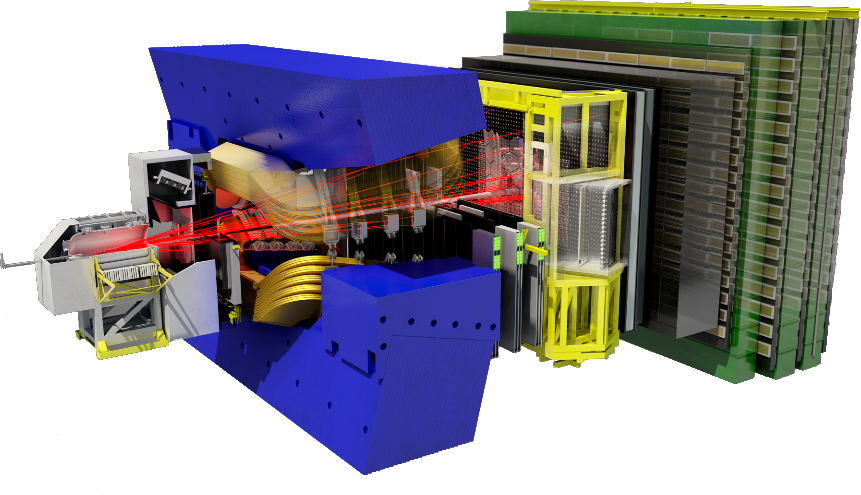
\includegraphics[width=\textwidth, trim=18 0 18 0]{images/LHCbDet.png}
  \end{center}
  \end{columns}

  \vspace{1em}
  \begin{center}
    \textbf{We need to rethink our algorithms from the ground up...}
  \end{center}
\end{frame}
